% Created 2022-01-24 Mon 19:07
% Intended LaTeX compiler: pdflatex
\documentclass[11pt]{article}
\usepackage[utf8]{inputenc}
\usepackage[T1]{fontenc}
\usepackage{graphicx}
\usepackage{longtable}
\usepackage{wrapfig}
\usepackage{rotating}
\usepackage[normalem]{ulem}
\usepackage{amsmath}
\usepackage{amssymb}
\usepackage{capt-of}
\usepackage{hyperref}
\usepackage{tikz}
\usetikzlibrary{arrows,shapes,snakes,automata,backgrounds,petri,positioning}
\usepackage{svg}
\author{Juan Escamilla Molgora, Luigi Sedda, Peter Diggle, Peter Atkinson}
\date{\today}
\title{A users' guide to apply the presence-only joint distribution framework for single species}
\hypersetup{
 pdfauthor={Juan Escamilla Molgora, Luigi Sedda, Peter Diggle, Peter Atkinson},
 pdftitle={A users' guide to apply the presence-only joint distribution framework for single species},
 pdfkeywords={},
 pdfsubject={},
 pdfcreator={Emacs 27.1 (Org mode 9.6)}, 
 pdflang={English}}
\begin{document}

\maketitle
\begin{abstract}
This document is a guide to use the models described in the paper: \emph{A joint distribution framework to improve presence-only species distribution models by exploiting opportunistic surveys} (\cite{EscamillaMolgora2021}) for modelling species distributions with presence-only data. This users' guide represents a static version. For an updated (and possibly improved) version, refer to the interactive Jupyter notebook at [\url{https://github.com/molgor/CAR-1SDM/blob/master/CAR-1SDM/notebooks/Users-guide.ipynb}].
\end{abstract}

The presented framework proposes three bayesian models for inferring single species distributions using solely observations of species occurrences (i.e. presence-only data).
The fundamental idea of the framework is that the observed occurrences (\(Y\)) are determined not only by the environmental conditions (niche) suitable for the species to thrive but also accounts for the bias in which these observations were collected (i.e. sampling effort). As such, the occurrences are specified as realisations of a join process composed of environmental conditions (\(P_Y\)) and sampling effort (\(P_X\)). These two components are explicitly defined with a model-based approach (\cite{Diggle2002}) to specify two types of covariates, one for \(P_X\) and other for \(P_Y\).
Both processes are specified as mixed models. That is, they are composed of  a fixed effect (i.e. \(E(P_X) = g(d_X;\beta_X)\) and \(E(P_Y) = g(d_Y;\beta_Y)\)) and a random effect that models the variation between observations across space. For the purposes of this example (and the presented results in the manuscript) we consider \(g(d_X;\beta_X)\) to be linear, that is: \(g(d_X;\beta_X) = \beta_X^t d_X\), where \(d_X\) is the vector of covariates associated to a given observation. For a clear description of the model refer to the manuscript and, specifically, to the supplementary materials.

The dependencies between processes \(P_X\) and \(P_Y\) are specified in terms of the covariance between all observations. That is, by their random effects; \(R_X\) and \(R_Y\) respectively. We proposed three forms to model these dependencies. Model I assumes \(R_X\) and \(R_Y\) are independent. Model II assumes that \(R_X = R_Y\) and Model III assumes both random effects are correlated. The three models specify a conditional autoregressive (CAR) (\cite{Besag1974}) model for defining the spatial random effect. Therefore, this framework is only suited for data aggregated in areas tilled over a region (i.e. spatial lattices).

In the following sections we will apply models I, II and III in the \textbf{R} programming language using the package CARBayes (\cite{Lee2013}). The data used was obtained from GBIF using the dataset (\cite{gbifmexdata}). This document is intended to serve as a guide for modelling species distributions using the aforementioned framework. For further reference of the Bayesian methodologies, diagnoses and deeper analysis of lattice-based models refer to (\cite{Lee2013,Rue2005})

\section{Model I}
\label{sec:org0a3b132}

This model assumes that the ecological suitability distribution (\(Y\)) and sampling effort \(X\) process are independent. The structure of the model is visualised as a directed acyclic graph (DAG) in the figure \ref{fig:M1}.  For a detail explanation of the model refer to the supplementary materials of the manuscript.

\begin{figure}
\label{fig:M1}
\centering
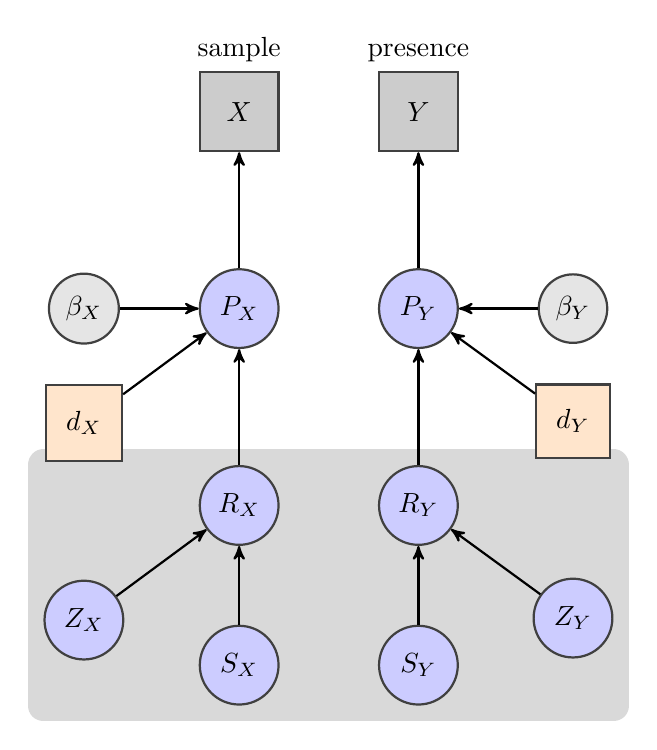
\begin{tikzpicture}[node distance=2.5cm,>=stealth',bend angle=45]
  \tikzstyle{latent}=[circle,thick,draw=black!75,fill=blue!20,minimum size=10mm]
  \tikzstyle{data}=[regular polygon,regular polygon sides=4,thick,draw=black!75,fill=orange!20,minimum size=7mm]
  \tikzstyle{parameter}=[latent,fill=gray!20,minimum
  size=7mm]
  \tikzstyle{obs}=[rectangle,thick,draw=black!75,fill=black!20,minimum size=10mm]
  \tikzstyle{null}=[]
  \tikzstyle{every label}=[black]

  \begin{scope}
    % First net
    \node [obs,label={above:sample}](X)    {$X$};
    \node [null](nulltop) [right = 0.5cm of X] {};
    \node [null](nullmid) [below of=nulltop] {};
    \node [null](nulldow) [below of=nullmid] {};
    \node [obs,label={above:presence}] (Y)  [right = 0.5cm of nulltop]  {$Y$};
    \node [latent] (Py) [below of=Y] {$P_Y$};
    \node [latent] (Px) [below of=X] {$P_X$};
    \node [parameter] (betax) [left = 1cm of Px] {$\beta_X$};
    \node [parameter] (betay) [right = 1cm of Py] {$\beta_Y$};
    \node [data]   (dx) [below = 0.5cm  of betax] {$d_X$};
    \node [data]   (dy) [below = 0.5cm of betay] {$d_Y$};
    \node [latent] (Rx) [below of=Px] {$R_X$};
    \node [latent] (Ry) [below of=Py] {$R_Y$};
    \node [latent] (Sx) [below = 1cm of Rx]
      {$S_X$};
    \node [latent] (Sy) [below = 1cm of Ry]
      {$S_Y$};
    \node [latent] (Zy) [below of=dy] {$Z_Y$};
    \node [latent] (Zx) [below of=dx] {$Z_X$};
    \end{scope}


      \begin{scope}
        \path [->, thick] (Px) edge node {} (X);
        \path [->, thick] (Py) edge node {} (Y);
        \path [->, thick] (Ry) edge node {}(Py);
        \path [->, thick] (Rx) edge node {} (Px);
        \path [->, thick] (Sx) edge (Rx);
        \path [->, thick] (Sy) edge (Ry);
        \path [->, thick] (Zx) edge (Rx);
        \path [->, thick] (Zy) edge (Ry);
        \path [->, thick] (betax) edge (Px);
        \path [->, thick] (dx) edge (Px);
        \path [->, thick] (betay) edge (Py);
        \path [->, thick] (dy) edge (Py);
      \end{scope}


      \begin{pgfonlayer}{background}
    \filldraw [line width=4mm,join=round,black!15]
        (Rx.north -| Zx.west)  rectangle (Sy.south
        -| Zy.east);
      %  (w1'.north -| l1'.east) rectangle (w2'.south -| e1'.west);
    \end{pgfonlayer}
\end{tikzpicture}
\caption{DAG for model I}
\end{figure}

\subsection{Running the model}
\label{sec:orge28e344}
We begin by defining the formulas for the sampling effort (formula\textsubscript{sample}) and the environmental niche (formula\textsubscript{presence}).
As we are dealing with only presence-absence realisations, we define a bernoulli process. That is, a binomial distribution with \(k=1\).
This can be specified with a 'trials' vector built on only ones.
\begin{verbatim}
formula_sample=sample~Disttoroadm+Populationm
formula_presence=species~Elevationm+MeanTempm
n <- nrow(TDF)
trials <- rep(1,n)
\end{verbatim}

We define the running settings for sampling the posterior distribution. In this case we specify 1,000 iterations after burnin (i.e. initialisation to reach stationarity of the Markov chain) of 70,000. To reduce hoarding data in memory we choose a thinning of 10. The postburnin parameter defines the number of iterations after burnin for each process but before saving the final sample of 1,000 iterations. Postburnin defines and extra burn-in iterations.
\begin{verbatim}
n.sample = 100000
burnin=70000
thin = 10
postburnin = burnin + 10000

model1  <- joint.binomial.bymCARModel1(formula_S = formula_sample,
                                        formula_P = formula_presence,
                                        n.sample=n.sample,
                                        data = DataFrame,
                                        burnin=burnin,
                                        postburnin=postburnin,
                                        thin=thin,
                                        verbose=TRUE)
\end{verbatim}

In model I, the processes \(S\) (sample) and \(P\) (environment) are independent. The object model1 contains these independent components stored as attributes S and P respectively. To inspect the posterior summary statistics we can use the attribute summary.results on each process.

\begin{verbatim}
model1$P$summary.results
\end{verbatim}

\begin{center}
\begin{tabular}{lrrrrrrr}
 & Median & 2.5\% & 97.5\% & n.sample & \% accept & n.effective & Geweke.diag\\
\hline
(Intercept) & -14.6010 & -22.0458 & -5.6759 & 10000 & 46.6 & 66.8 & 1.4\\
Elevationm & 0.0016 & 0.0000 & 0.0031 & 10000 & 46.6 & 83.1 & 0.5\\
 &  &  &  &  &  &  & \\
MeanTempm & -0.0428 & -0.3228 & 0.2136 & 10000 & 46.6 & 104.9 & 0.6\\
 &  &  &  &  &  &  & \\
tau2 & 6.9339 & 3.8265 & 15.0163 & 10000 & 100.0 & 45.5 & -1.1\\
 &  &  &  &  &  &  & \\
sigma2 & 0.0312 & 0.0029 & 0.3400 & 10000 & 100.0 & 8.1 & 1.4\\
\end{tabular}
\end{center}

\subsection{Modelfit statistics}
\label{sec:org2747ae5}
Model fitting criteria can be inspected with the argument (modelfit). Available statistics are:
Deviance information criteria (DIC), Watanabe-Akaike information Criterion (WAIC), log marginal predictive likelihood (LMPL), estimated effective number of parameters (p.d.) and  loglikelihood.

\begin{verbatim}
model1$summary.results #For general modelfit of both models simultaneously.
model1$P$modelfit
model1$S$modelfit
\end{verbatim}

\subsection{Convergence of the Markov chain by visual inspection}
\label{sec:org265df21}
\begin{verbatim}
library(coda)
params.samples <- mcmc.list(model1$P$samples$beta)
plot(params.samples)
\end{verbatim}

\begin{figure}[htbp]
\centering
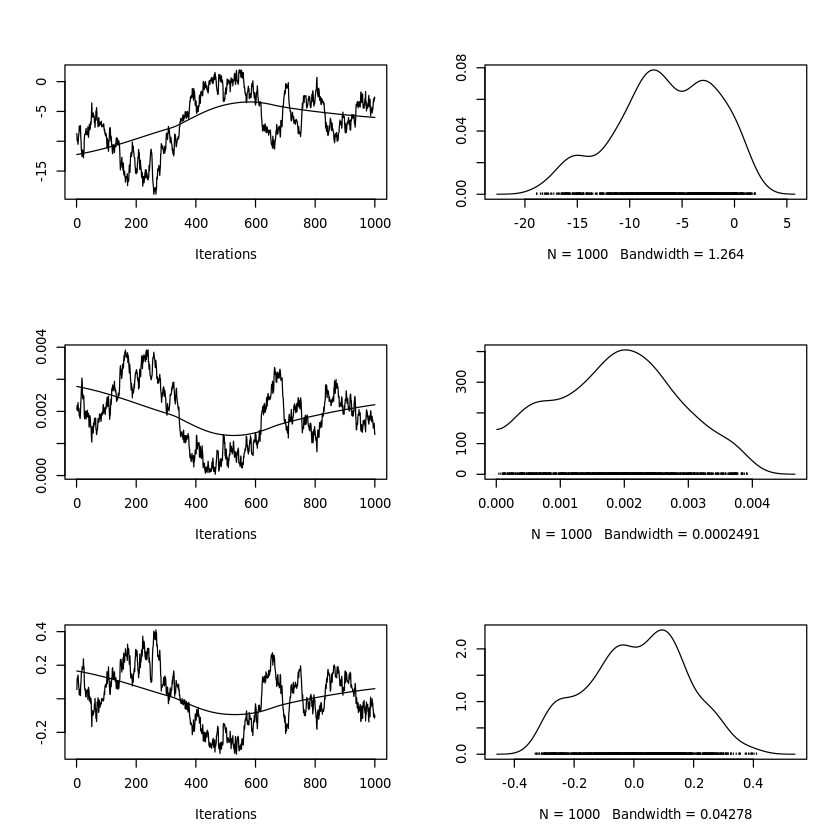
\includegraphics[width=.9\linewidth]{./traceplot.png}
\caption{Traceplot of posterior distribution of parameters for Model I}
\end{figure}



\subsection{Cross-validation}
\label{sec:org86a5da8}
In this subsection we will perform a cross-validation of model I. Cross validation of CAR models is not straight forward due to its spatial structure (lattice). The approach for this would be with data augmentation and the k-fold method (\cite{Geisser1975}). In this case we will randomly (without replacement) select 1/10 of the observations (sites) as missing data, fit the model, estimate the probability of \(Y\) and \(X\) on these sites and repeat this operation 10 times until we obtain a whole set of estimated observations. Afterwards we will calculate the the Receiver Operator Characteristic and its Area Under the Curve (i.e. AUC-ROC, also called ROC-curve).

We will load the script init\textsubscript{data.R}

\subsection{Setting the working directory.}
\label{sec:org9dc427d}
Change accordingly to your installation.

\begin{verbatim}
setwd('/main/app/external_plugins/biospytial_rwrapper/CAR-1SDM/')
source('R/preprocess_data.R')
# load Model 1
source("joint.binomial.bymCARModel1.R")
\end{verbatim}

A brief data exploration shows the number of relative absences and presences (npresence\textsubscript{0,npresece}\textsubscript{1}) in the ``presences'' process \(Y\), the in the sampling process \(X\)  (i.e. nsample\textsubscript{0} and nsample\textsubscript{1}, respectively). Missed data (no observations) are shown as n\textsubscript{miss}\textsubscript{presence} and n\textsubscript{miss}\textsubscript{sample}. for \(Y\) and \(X\) respectively.

\begin{verbatim}
ntot = length(DataFrame$sample)
npresence_1 = length(na.omit(DataFrame$species[DataFrame$species == 1])) / ntot*100
nsample_1 = length(na.omit(DataFrame$sample[DataFrame$sample == 1]))/ntot*100
npresence_0 = length(na.omit(DataFrame$species[DataFrame$species == 0]))/ntot*100
nsample_0 = length(na.omit(DataFrame$sample[DataFrame$sample == 0]))/ntot*100
n_miss_presence = sum(is.na(DataFrame$species))/ntot*100
n_miss_sample = sum(is.na(DataFrame$sample))/ntot*100
cbind(npresence_0,npresence_1,nsample_0,nsample_1,n_miss_presence,n_miss_sample)
\end{verbatim}

\begin{verbatim}
     npresence_0 npresence_1 nsample_0 nsample_1 n_miss_presence n_miss_sample
[1,]    63.02956    8.399015  10.59113  71.42857        28.57143       17.9803
\end{verbatim}


\subsection{Preparing the cross-validation}
\label{sec:orgb25c04d}
\begin{enumerate}
\item We begin by loading necessary packages:
\begin{verbatim}
    library(pROC)
    library('caret')
\end{verbatim}

\item Create partitions for cross validation using the K-fold method (k=7) and prepare the dataframe to receive results.
\begin{verbatim}
      nonas = which(! is.na(DataFrame$species) )
      Y_withoutNA = DataFrame$species[nonas]
      validate = createFolds(y = Y_withoutNA, k=7, returnTrain = FALSE)
      DataFrame$presences <- DataFrame$species
      l <- list()
      i = 1
      DataFrame$predicted_values_CV <- NA
      DataFrame$predicted_valuesBernoulli <- NA
\end{verbatim}

\item Define the formulas for the presence (environmental) process \(Y\) and the sampling effort \(X\)
\begin{verbatim}
     formula_sample =  sample ~ Disttoroadm + Populationm
     formula_presence = species ~ Elevationm + Precipitationm
\end{verbatim}

\item Cross validation
\begin{itemize}
\item First we define the parameters for sampling the posterior distribution (MCMC).
\end{itemize}
\begin{verbatim}
     n.sample = 20000
     burnin=15000
     postburnin = burnin + 1000
\end{verbatim}
\begin{itemize}
\item Perform the cross-validation
\end{itemize}
\begin{verbatim}
     for (fold in validate) {
       observed.presences <- DataFrame$species[fold]
       ## Substitue by NA
       DataFrame$species[fold] <- NA
       results  <- joint.binomial.bymCARModel1(formula_S = formula_sample,
                                formula_P = formula_presence,
                                n.sample=n.sample,
                                data = DataFrame,
                                burnin=burnin,
                                postburnin=postburnin,
                                thin=thin,
                                verbose=TRUE)

       DataFrame$species <- DataFrame$presences
       ## Return original values
       DataFrame$predicted_values_CV[fold] <- results$fitted.values[fold]
       predicted.probability = results$fitted.values[fold]

    ## Generate Bernoulli sample [ Only for the fold data set]
    print("Generating bernoulli sampling...")
    post.joint = data.frame(results$samples$fitted.joint[fold])
    ptot <- post.joint %>% mutate_all(function(p) rbernoulli(1,p))
    sumpt <- colSums(ptot)
    nsamples = dim(ptot)[1]
    ProbPS <- sumpt / nsamples

    DataFrame$predicted_valuesBernoulli[fold] <- ProbPS
    i = i + 1
}
\end{verbatim}
\end{enumerate}

\subsubsection{Plot the RO curve}
\label{sec:org19afc88}
\begin{verbatim}
pROC_obj <- roc(DataFrame$presences,DataFrame$predicted_values_CV,
               smoothed= TRUE,
               ci = TRUE, ci.alpha=0.9, stratified=FALSE,
               plot=TRUE, auc.polygon=TRUE, max.auc.polygon=TRUE, grid=TRUE,
               print.auc=TRUE, show.thres=TRUE)
sens.ci <- ci.se(pROC_obj)
plot(sens.ci,type="shape",col="lightblue")
plot(sens.ci, type="bars")
\end{verbatim}

Figure 3 shows the resulting output.

Procedure for cross-validating models II and III can be performed similarly.

\begin{figure}[htbp]
\centering
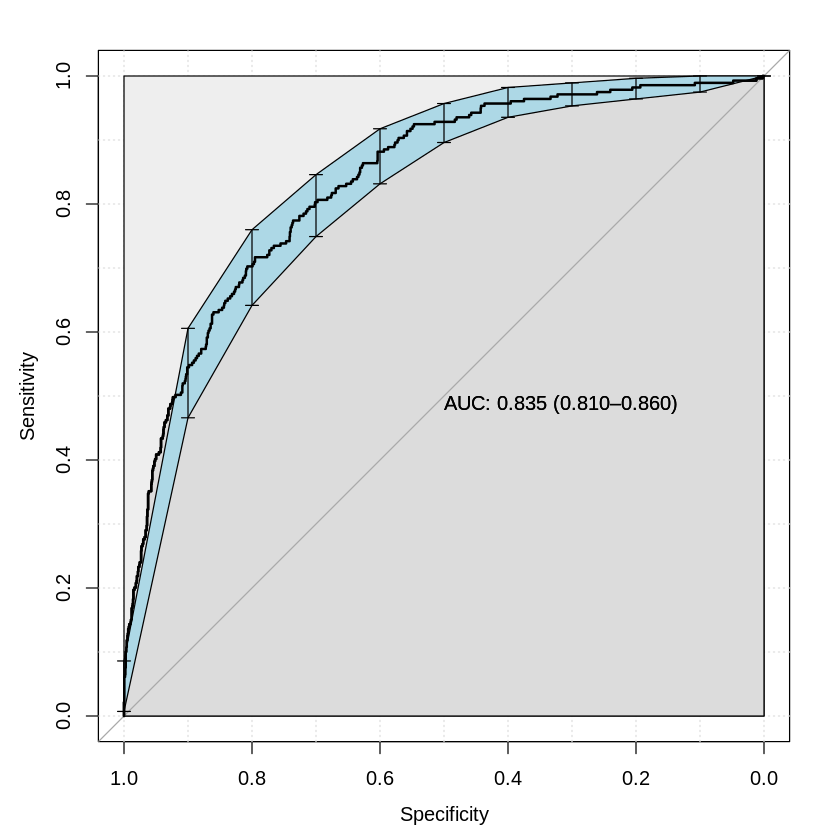
\includegraphics[width=.9\linewidth]{./rocmodel1wNA.png}
\caption{Resulting cross-validation curve}
\end{figure}


\section{Model II}
\label{sec:orgb360ba3}
This model assumes that the ecological suitability distribution (\(P\)) and sampling effort (\(S\)) processes are independent when conditioned to a common spatial structure (\(G\)) (a Gaussian Markov random field). The structure of the model is visualised as a directed acyclic graph (DAG) in the figure \ref{fig:M2}.  For a detail explanation of the model refer to the supplementary materials of the manuscript.

\begin{figure}
\label{fig:M2}
\centering
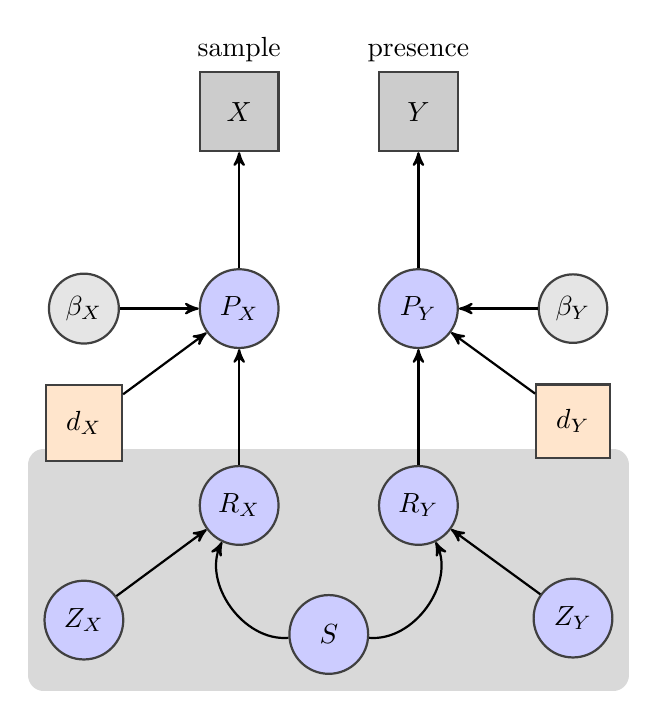
\begin{tikzpicture}[node distance=2.5cm,>=stealth',bend angle=45]
  \tikzstyle{latent}=[circle,thick,draw=black!75,fill=blue!20,minimum size=10mm]
  \tikzstyle{data}=[regular polygon,regular polygon sides=4,thick,draw=black!75,fill=orange!20,minimum size=7mm]
  \tikzstyle{parameter}=[latent,fill=gray!20,minimum
  size=7mm]
  \tikzstyle{obs}=[rectangle,thick,draw=black!75,fill=black!20,minimum size=10mm]
  \tikzstyle{null}=[]
  \tikzstyle{every label}=[black]

  \begin{scope}
    % First net
    \node [obs,label={above:sample}](X)    {$X$};
    \node [null](nulltop) [right = 0.5cm of X] {};
    \node [null](nullmid) [below of=nulltop] {};
    \node [null](nulldow) [below of=nullmid] {};
    \node [obs,label={above:presence}] (Y)  [right = 0.5cm of nulltop]  {$Y$};
    \node [latent] (Py) [below of=Y] {$P_Y$};
    \node [latent] (Px) [below of=X] {$P_X$};
    \node [parameter] (betax) [left = 1cm of Px] {$\beta_X$};
    \node [parameter] (betay) [right = 1cm of Py] {$\beta_Y$};
    \node [data]   (dx) [below = 0.5cm  of betax] {$d_X$};
    \node [data]   (dy) [below = 0.5cm of betay] {$d_Y$};
    \node [latent] (Rx) [below of=Px] {$R_X$};
    \node [latent] (Ry) [below of=Py] {$R_Y$};
    \node [latent] (S) [below = 1cm of nulldow] {$S$};
    \node [latent] (Zy) [below of=dy] {$Z_Y$};
    \node [latent] (Zx) [below of=dx] {$Z_X$};
    \end{scope}


      \begin{scope}
        \path [->, thick] (Px) edge node {} (X);
        \path [->, thick] (Py) edge node {} (Y);
        \path [->, thick] (Ry) edge node {}(Py);
        \path [->, thick] (Rx) edge node {} (Px);
        \path [->, thick] (S) edge [bend left=60] (Rx);
        \path [->, thick] (S) edge [bend right=60] (Ry);
        \path [->, thick] (Zx) edge (Rx);
        \path [->, thick] (Zy) edge (Ry);
        \path [->, thick] (betax) edge (Px);
        \path [->, thick] (dx) edge (Px);
        \path [->, thick] (betay) edge (Py);
        \path [->, thick] (dy) edge (Py);
      \end{scope}

    \begin{pgfonlayer}{background}
    \filldraw [line width=4mm,join=round,black!15]
        (Rx.north -| Zx.west)  rectangle (S.south
        -| Zy.east);
    \end{pgfonlayer}
\end{tikzpicture}
\caption{DAG for model II}
\end{figure}

\subsection{Running the model}
\label{sec:org4790ff1}
To run the model we first need to transform the data, specifically, the covariates matrix (i.e. design matrix). The transformation allows the fitting of specific covariates for each process (i.e. an environmental set of covariates and another set for the sampling effort).

To do this, we stack the design matrices of \(S\) and \(P\) and extend the number of columns to the sum of both processes.
That is, the number of columns of the resulting matrix is the sum of the columns of \(P\) and \(S\) (not counting the response variables). We begin by selecting the covariates for each process following a standard formula syntax (one formula per process).

\begin{verbatim}
formula_sample =  sample ~ Disttoroadm + Populationm
formula_presence = species ~ Elevationm + Precipitationm


## Build dataframes, S <- Sample, P <- Presence
S <- model.frame(formula_sample, DataFrame,na.action='na.pass')
P <- model.frame(formula_presence, DataFrame,na.action='na.pass')

## Split response variables (lefthand side) and covariates (righthand side)
## from the design matrix
SX <- select(S, -c(1))
PX <- select(P, -c(1))
Sy <- select(S, c(1))
Py <- select(P, c(1))

## Assign names to columns
names(Sy) <- 'response'
names(Py) <- names(Sy)

## Stack both processes into same dataframe
## First the responses (Y) will be concatenated by row.
Y = rbind(Sy,Py)
\end{verbatim}

To join both sets of covariates (SX and PX) into the stacked design matrix, we need to join the columns of SX and PX. As there's no information of environmental variables for process S and, viceversa, no information of the sampling covariates for process P, we assign 0 to these elements.

For doing this, we first define two 2x2 matrices and perform the kronnecker product to generate a block diagonal design matrix to be used as the covariates of the stacked design matrix.

\begin{verbatim}

T1 <- matrix(rep(0,4), ncol = 2)
T2 <- matrix(rep(0,4), ncol = 2)
T1[1,1] <- 1
T2[2,2] <- 1

## Perform Kronnecker with different covariates (Block diagonal)
X <- data.frame((T1 %x% as.matrix(SX)) + (T2 %x% as.matrix(PX)))
names(X) <- c(names(SX),names(PX))

## Lastly, we bind the stacked response variable with the stacked covariance matrix.
SDM <- cbind(Y,X)
\end{verbatim}

\subsection{Defining other necessary arguments}
\label{sec:org58b509c}
\begin{verbatim}
## Get number of elements in the lattice,
nK <- dim(M_bis)[1]

## make sequence vector for id.area
## This is possible because the rows in adjacency matrix M_bis preserve the
## order of each element in the design matrix.
ida <- data.frame(seq(nK))
idarea <- unlist(rbind(ida,ida))
## Assign values for the unstructured random effect (Zx, Zy).
## In this case, all elements of S share the same random effect Zx.
## Similarly, all elements of P share the same random effect Zy.
## This is done with
Zx <- rep(x = 1,times = nK)
Zy <- rep(x = 2,times = nK)
## Stack Zx and Zy to create a vector of labels used to define
## the unstructured random effect.
indre <- c(Zx,Zy)
\end{verbatim}

\subsection{Running the model}
\label{sec:orgf718d66}
\begin{verbatim}
#formula_sample =  sample ~ Disttoroadm + Populationm
#formula_presence = species ~ Elevationm + Precipitationm
formula <- response ~ Disttoroadm + Populationm
                      + Elevationm + Precipitationm
ind.re = c(rep(1,nK),rep(2,nK))

ntot <- dim(SDM)[1]
trials <- rep(1,ntot)
## uncomment for real testing
#burnin = 1000000
#n.sample = 1200000
#thin = 50
## Toy example
burnin = 100
n.sample = 120
thin = 1

model2 <- S.CARmultilevel(formula,family = 'binomial',
                          trials=as.numeric(trials),
                          W=M_bis,
                          ind.area=idarea,
                          #ind.re=factor(idarea),
                          ind.re = factor(ind.re),
                          rho=1,
                          burnin=burnin,
                          n.sample=n.sample,
                          data=SDM)
\end{verbatim}

Similarly to model I, the posterior summary statistics can be inspected by accessing the attribute summary.results.

\begin{verbatim}
model2$P$summary.results
\end{verbatim}

\section{Model III}
\label{sec:org959c3de}
This model assumes that processes \(S\) and \(P\) are correlated to each other. Both of them have a specific Gaussian Markov random field and these two spatial structures are correlated. The correlated spatial structure follows a multivariate CAR specification (\cite{kavanagh2016,Lee2013}). The structure of the model is visualised as a directed acyclic graph (DAG) in the figure \ref{fig:M3}.  For a detail explanation of the model refer to the supplementary materials of the manuscript.
The joint probability distribution of \(P\) and \(S\) is given by:
 $$ [P , S ] = [P | GMRF_p] [ S | GMRF_s] $$
\begin{figure}
\label{fig:M3}
\centering
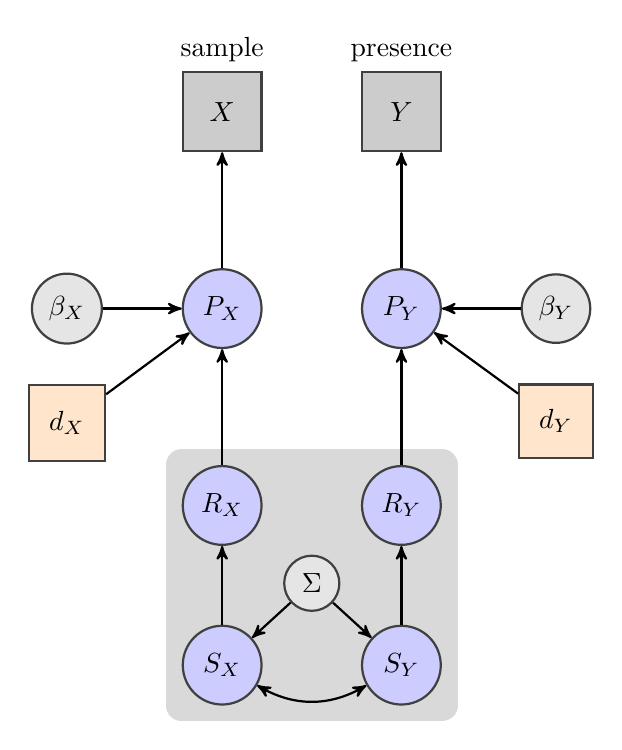
\begin{tikzpicture}[node distance=2.5cm,>=stealth',bend angle=45]
  \tikzstyle{latent}=[circle,thick,draw=black!75,fill=blue!20,minimum size=10mm]
  \tikzstyle{data}=[regular polygon,regular polygon sides=4,thick,draw=black!75,fill=orange!20,minimum size=7mm]
  \tikzstyle{parameter}=[latent,fill=gray!20,minimum
  size=7mm]
  \tikzstyle{obs}=[rectangle,thick,draw=black!75,fill=black!20,minimum size=10mm]
  \tikzstyle{null}=[]
  \tikzstyle{every label}=[black]

  \begin{scope}
    % First net
    \node [obs,label={above:sample}](X)    {$X$};
    \node [null](nulltop) [right = 0.5cm of X] {};
    \node [null](nullmid) [below of=nulltop] {};
    \node [null](nulldow) [below of=nullmid] {};
    \node [obs,label={above:presence}] (Y)  [right = 0.5cm of nulltop]  {$Y$};
    \node [latent] (Py) [below of=Y] {$P_Y$};
    \node [latent] (Px) [below of=X] {$P_X$};
    \node [parameter] (betax) [left = 1cm of Px] {$\beta_X$};
    \node [parameter] (betay) [right = 1cm of Py] {$\beta_Y$};
    \node [data]   (dx) [below = 0.5cm  of betax] {$d_X$};
    \node [data]   (dy) [below = 0.5cm of betay] {$d_Y$};
    \node [latent] (Rx) [below of=Px] {$R_X$};
    \node [latent] (Ry) [below of=Py] {$R_Y$};
    \node [latent] (Sx) [below = 1cm of Rx] {$S_X$};
    \node [latent] (Sy) [below = 1cm of Ry] {$S_Y$};
    \node [parameter] (Sigma)[below = 0.5cm of nulldow]
      {$\Sigma$};
    %\node [latent] (Zy) [below of=dy] {$Z_Y$};
    %\node [latent] (Zx) [below of=dx] {$Z_X$};
    \end{scope}


      \begin{scope}
        \path [->, thick] (Px) edge node {} (X);
        \path [->, thick] (Py) edge node {} (Y);
        \path [->, thick] (Ry) edge node {}(Py);
        \path [->, thick] (Rx) edge node {} (Px);
        \path [->, thick] (Sx) edge (Rx);
        \path [->, thick] (Sy) edge (Ry);
        \path [<->, thick] (Sy) edge [bend left=30] (Sx);
        \path [->, thick] (Sigma) edge (Sx);
        \path [->, thick] (Sigma) edge (Sy);
        %\path [->, thick] (Zx) edge (Rx);
        %\path [->, thick] (Zy) edge (Ry);
        \path [->, thick] (betax) edge (Px);
        \path [->, thick] (dx) edge (Px);
        \path [->, thick] (betay) edge (Py);
        \path [->, thick] (dy) edge (Py);
      \end{scope}

    \begin{pgfonlayer}{background}
    \filldraw [line width=4mm,join=round,black!15]
        (Rx.north -| Sx.west)  rectangle (Sy.south
        -| Ry.east);
    \end{pgfonlayer}
\end{tikzpicture}
\caption{DAG for model III}
\end{figure}

\subsection{Running the model}
\label{sec:orgbc76aec}
Applying this model is straight forward. We only need to define an appropriate formula object.

\begin{verbatim}
formula <- cbind(species,sample) ~ Elevationm + Precipitationm +
                                   Disttoroadm + Populationm
## Get number areal elements
K <- dim(M_bis)[1]
## Calculate new trial vector
trials <- matrix(rep(1.0,K*2), ncol=2)

## Toy example, increase n.sample and burnin significantly for real applications.
burnin = 400
n.sample = 500
thin = 5
model3 <- MVS.CARleroux(formula ,
                        family = 'binomial',
                        trials=trials,
                        W=M_bis,
                        rho = 1,
                        burnin = burnin,
                        n.sample = n.sample,
                        data = DataFrame
                         )

\end{verbatim}

To examine the model diagnostics use modelfit, as usual.

\begin{verbatim}
model3$modelfit
\end{verbatim}

\begin{center}
\begin{tabular}{rrrrrr}
DIC & p.d & WAIC & p.w & LMPL & loglikelihood\\
\hline
3976.2 & 93.21 & 3966.76 & 81.39 & -1982.01 & -1894.88\\
\end{tabular}
\end{center}



\bibliographystyle{unsrt}
\bibliography{../../../../../../../texmf/bibtex/bib/library}
\end{document}
